\chapter{Desenvolvimento}

Diferente de muitos outras interfaces de desenvolvimento, o KDevelop permite o usuário incorporar qualquer projeto de software na IDE,
contando que siga alguns padrões já estabelecidos. Boa parte das configurações do projeto são obtidas na IDE para a configuração, vem dos gerenciadores de compilação.

\section{Ferramentas Utilizadas}
As seguintes ferramentas foram utilizadas para desenvolvimento do projeto.
\begin{itemize}
 \item \textbf{KDevelop}: Editor de código para desenvolvimento do plugin e na realização de debug.
 \item \textbf{QT}: Kit de ferramentas e bibliotecas para desenvolvimento de software.
 \item \textbf{KDE Framework}: Coleção de ferramentas e bibliotecas do KDE.
 \item \textbf{Avrdude}: Programa de carregamento de código para microcontroladores AVR.
 \item \textbf{OpenOCD}: Ferramenta para comunicação de programadores.
 \item \textbf{Placas de desenvolvimento}: Arduino mini, nano, mega, due, uno para testes de suporte utilizando avrdude. Stellaris LM4F232 para testes utilizando o OpenOCD.
\end{itemize}

Com o objetivo do trabalho de seguir a filosofia GNU \cite{filosofia}, todos as ferramentas utilizadas para o desenvolvimento do plugin são de código aberto e totalmente gratuitas para qualquer um que queira replicar, modificar e contribuir com o projeto.

\section{Desenvolvimento do software}

\begin{figure}[!htb]
  \centering
  \caption[UML proposto]{UML proposto para desenvolvimento do plugin.}
  \label{fig:uml}
  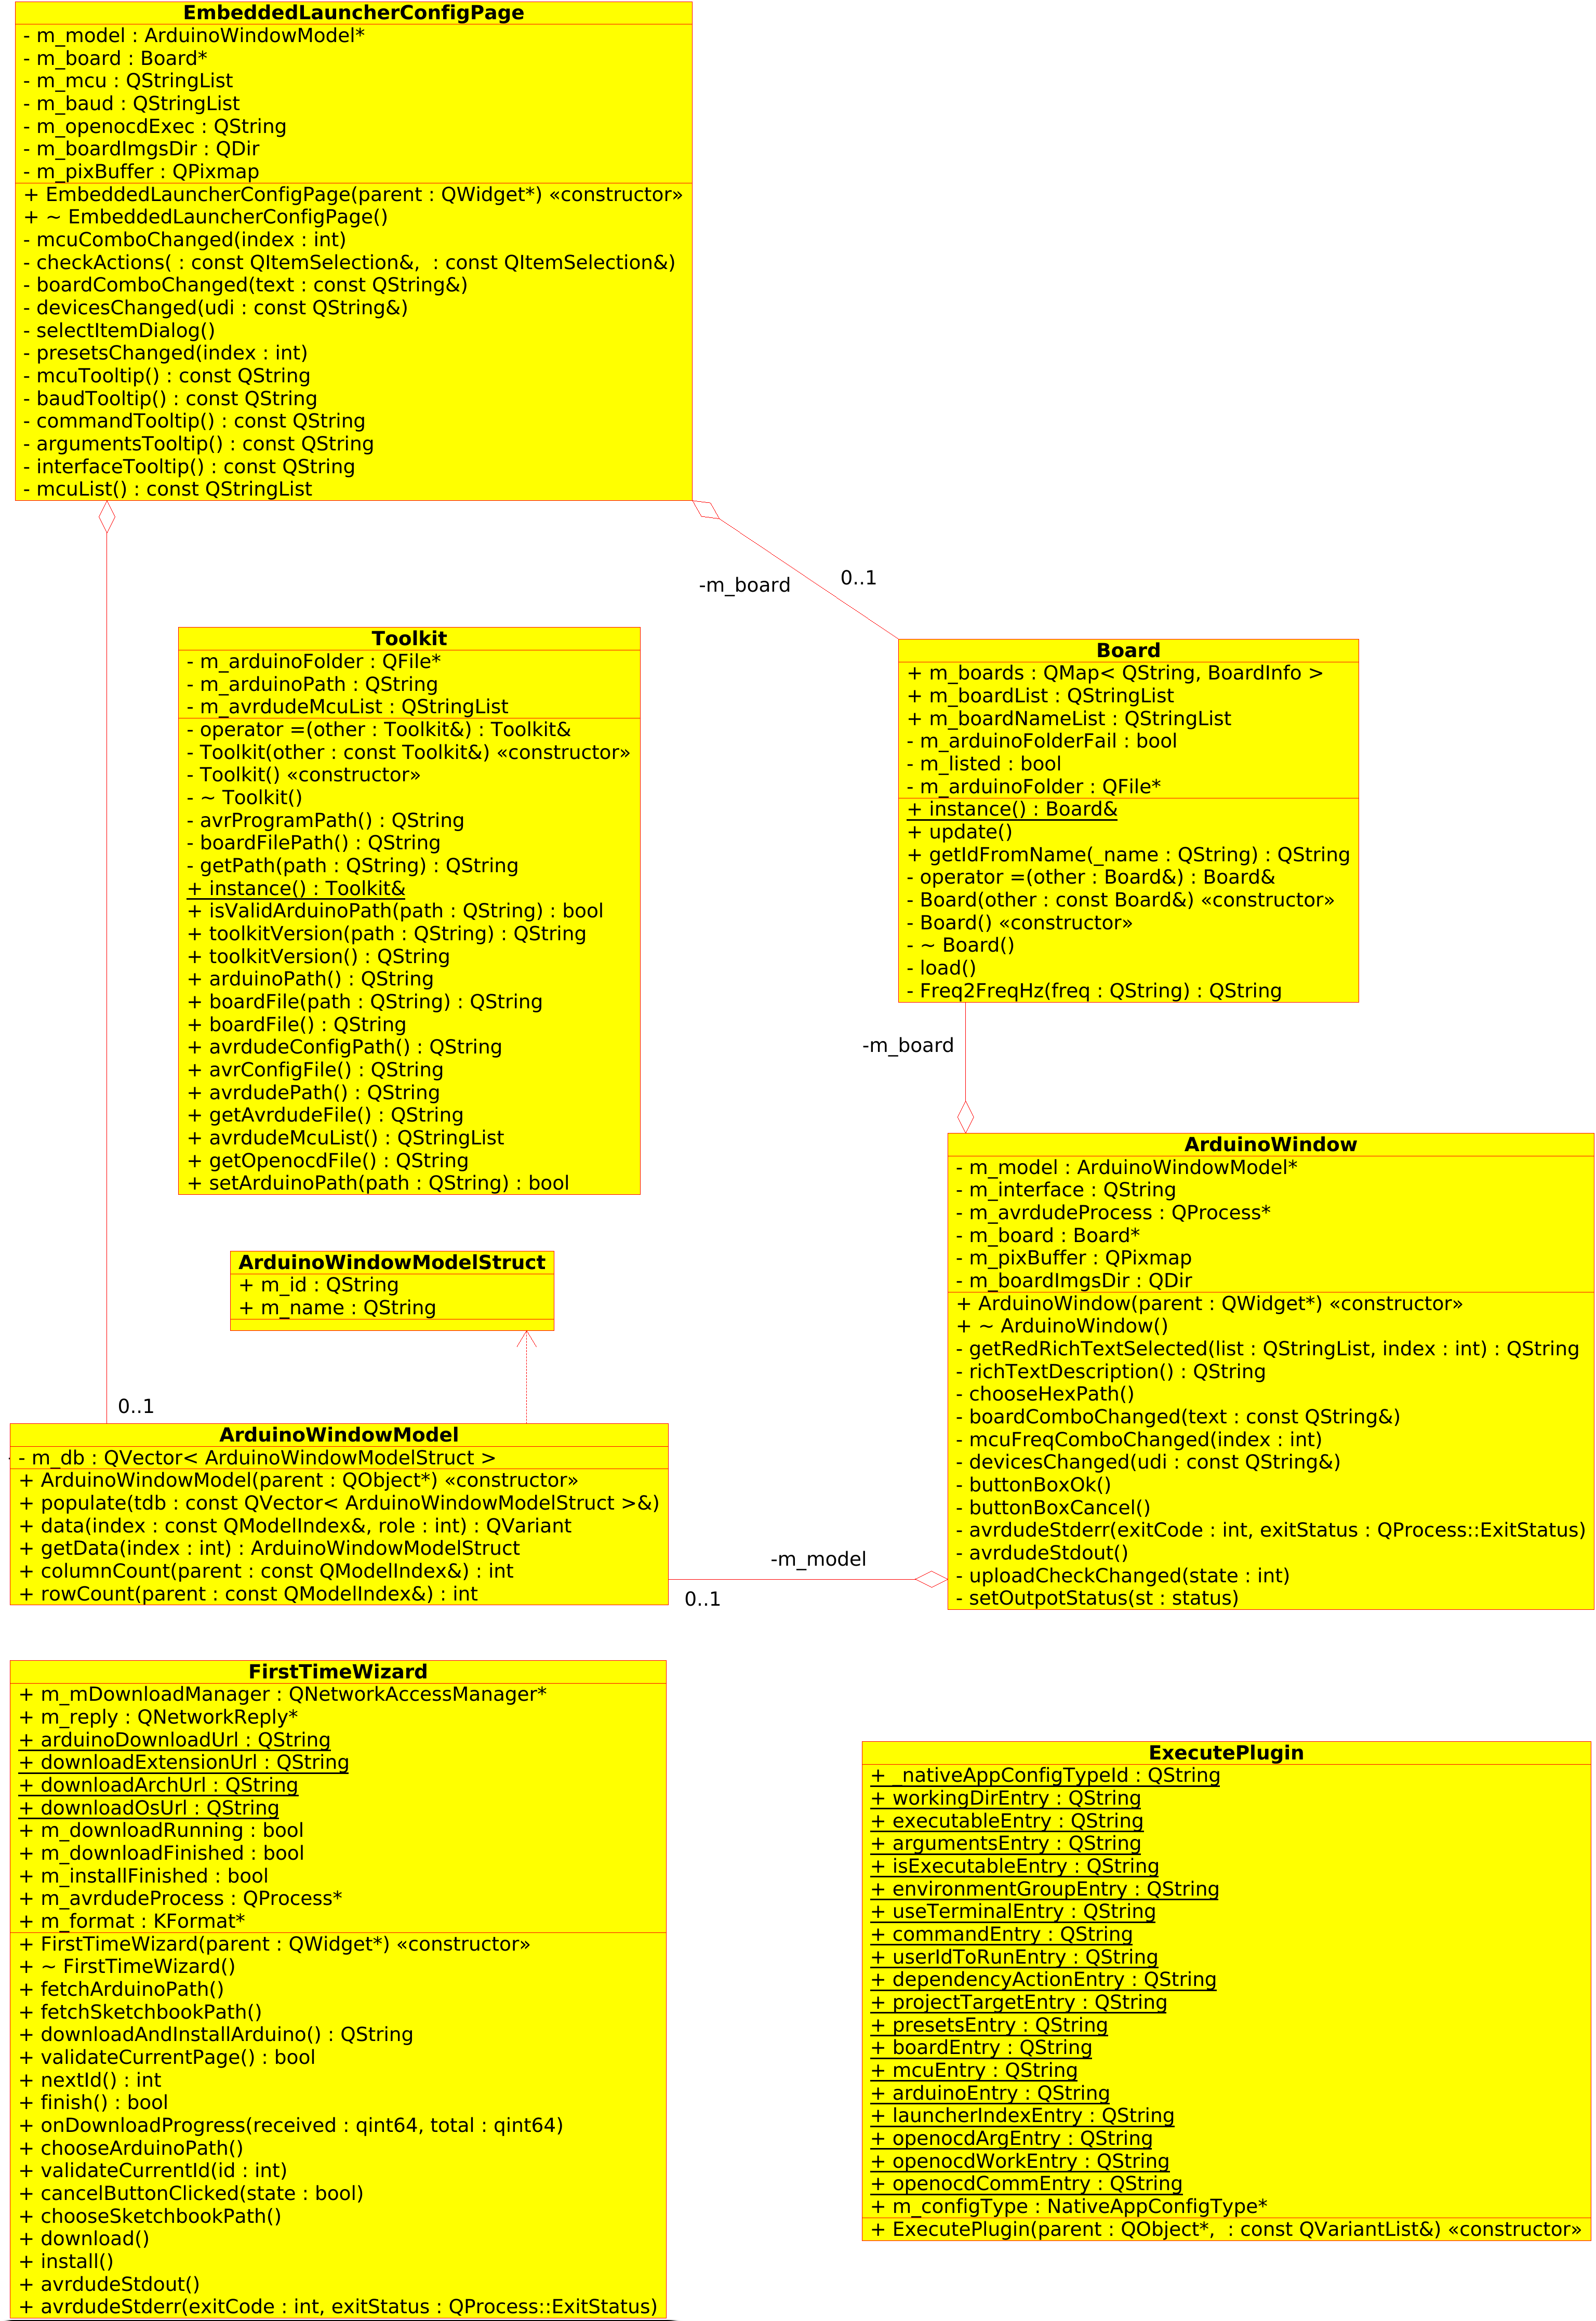
\includegraphics[width=0.85\textwidth]{figuras/uml.png}
\end{figure}

\abreviatura{UML}{Unified Modeling Language}

O plugin (\figref{fig:uml}) foi integrado no KDevelop (\figref{fig:kdevelop}) via a utilização de ferramentas básicas de desenvolvimento para o mesmo (\textit{kdevplatform}). Nesta seção, será demonstrando as interfaces desenvolvidas e sua integração com o KDevelop.

\begin{figure}[!htb]
  \centering
  \caption[KDevelop]{KDevelop.}
  \label{fig:kdevelop}
  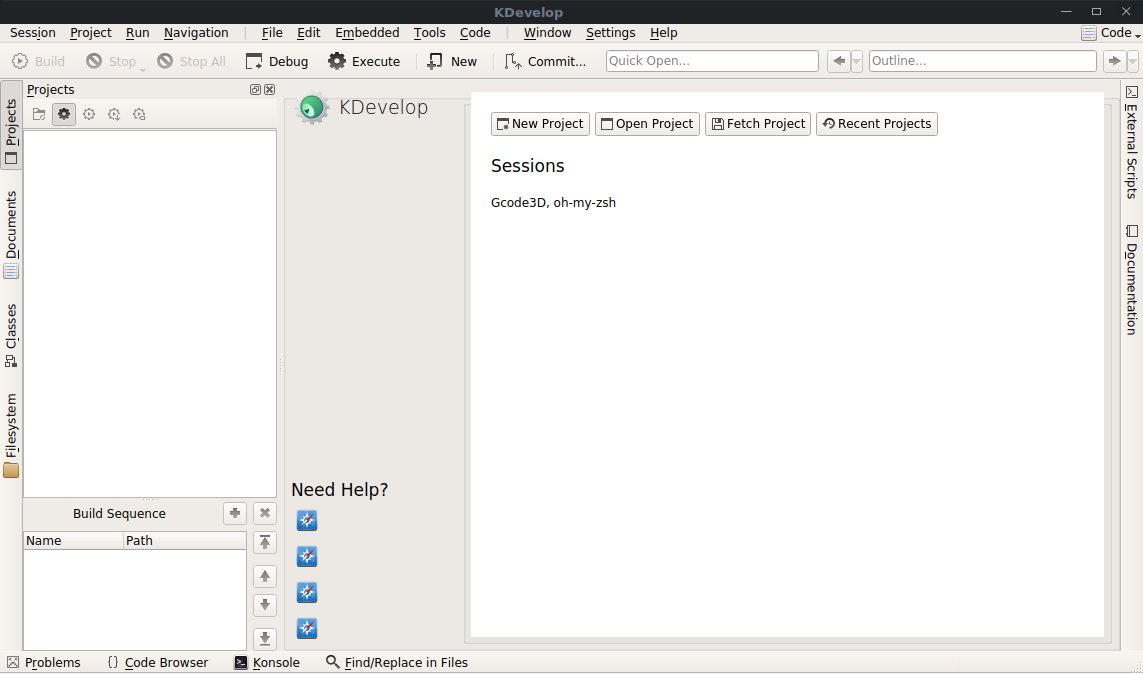
\includegraphics[width=0.85\textwidth]{figuras/kdevelop.png}
\end{figure}

\subsection{Menu de acesso}

O menu de acesso (\figref{fig:kdevelopMenu}), foi desenvolvido para realizar duas funções, configurar o plugin em relação as ferramentas necessárias para sua utilização com as placas da \textit{Arduino} (\textit{Arduino Setup}), e permitir a realização do carregamento de código desenvolvido para a placa, utilizando uma interface gráfica assistencialista (\textit{Board settings}).

\begin{figure}[!htb]
  \centering
  \caption[Menu do plugin no KDevelop]{Menu de acesso do plugin no KDevelop.}
  \label{fig:kdevelopMenu}
  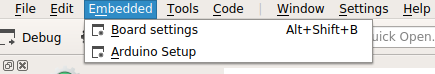
\includegraphics[width=0.95\textwidth]{figuras/kdevelopMenu.png}
\end{figure}

\subsection{Arduino Setup}

Realiza a configuração inicial do plugin no sistema, permitindo ao usuário escolher uma versão do kit de ferramentas do \textit{Arduino} para utilizar ou a instalação automática do kit pelo plugin.

Primeiramente foi definido um diagrama inicial de estados para facilitar a compreensão da configuração (\figref{fig:ftwstate}).

\begin{itemize}
\item \textbf{\textit{First-Time Configuration} (FTC)}: Tela inicial, permitindo ao usuário escolher o local do \textit{toolkit} previamente instalado (\figref{fig:kdevelopinstaller1}), ou escolher a opção de instalação automática. 

\item \textbf{\textit{Automatic Instalation} (AutoInst)}: Tela resultante da escolha da instalação automática na configuração inicial do \textbf{\textit{First-Time Configuration}}. Essa, separada em duas etapas, \textit{Download} e \textit{Install}.

\subitem \textbf{\textit{Download} (Down)}: É realizado a comunicação com o servidor oficial resultando no download das ferramentas necessárias (\figref{fig:kdevelopinstaller21}).

\subitem \textbf{\textit{Install}}: Após o \textit{download} é realizado a decomposição e instalação do conjunto de ferramentas (\figref{fig:kdevelopinstaller22}).

\item \textbf{\textit{End Configuration} (EndConf)}: Tela final, resulta após a escolha de um \textit{toolkit} previamente instalado ou após a conclusão da instalação automática (\figref{fig:kdevelopinstaller3}).
\end{itemize}

\begin{figure}[htb!]
  \centering
    \caption[Diagrama de estados do \textit{First-Time Wizard}]{Diagrama de estados do \textit{First-Time Wizard}}
    {\label{fig:ftwstate}}
  \begin{tikzpicture}[->,>=stealth',shorten >=1pt,auto,node distance=2.8cm,semithick]
    \tikzstyle{every state}=[fill=blue,draw=none,text=white]

	%First-Time Configuration
    \node[state]         (A)                    {$FirstTimeConf.$}; 
    % Automactic Install
    \node[state]         (B) [right of=A]       {$Auto Inst.$};
    \node[state]         (C) [right of=B]       {$Down.$};
    \node[state]         (D) [below of=C]       {$Install$};
    \node[state]         (E) [below of=A]       {$EndConf$};

    \path (A) edge              node {Existing Installation}      (E)
	      (A) edge  [bend left]   node {Automatic Installation}      (B)
          (B) edge              node {}      (C)
          (C) edge              node {}      (D)
          (D) edge              node {}      (E);
  \end{tikzpicture}
\end{figure}


\begin{figure}[!htb]
  \centering
  \caption[Fist-Time Configuration]{\textit{Fist-Time Configuration} com \textit{Existing Installation} selecionado.}
  \label{fig:kdevelopinstaller1}
  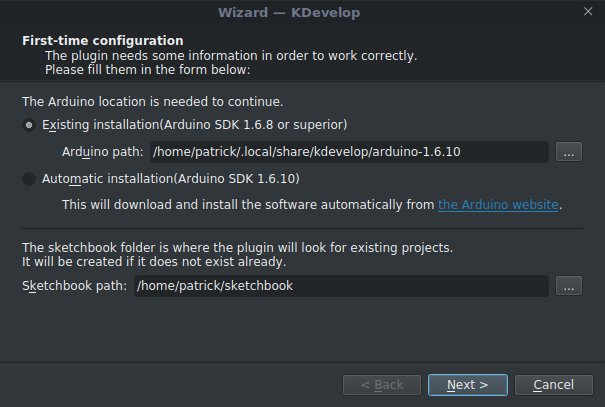
\includegraphics[width=0.85\textwidth]{figuras/kdevelopInstaller1.png}
\end{figure}

\begin{figure}[!htb]
  \centering
  \caption[Automatic Instalation executando Download]{\textit{Automatic Instalation} com \textit{download} em andamento.}
  \label{fig:kdevelopinstaller21}
  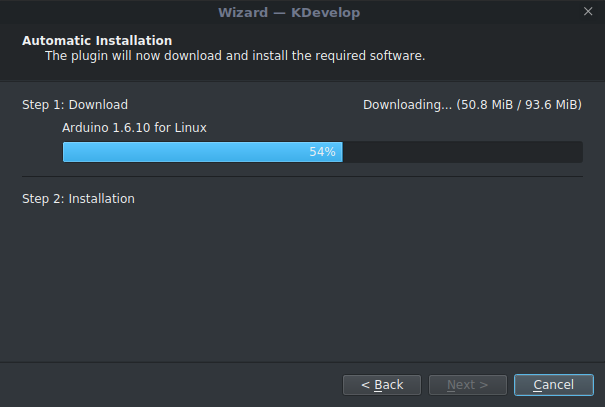
\includegraphics[width=0.85\textwidth]{figuras/kdevelopInstaller21.png}
\end{figure}

\begin{figure}[!htb]
  \centering
  \caption[Automatic Instalation pós instalação]{Automatic Instalation após a instalação do \textit{toolkit}.}
  \label{fig:kdevelopinstaller22}
  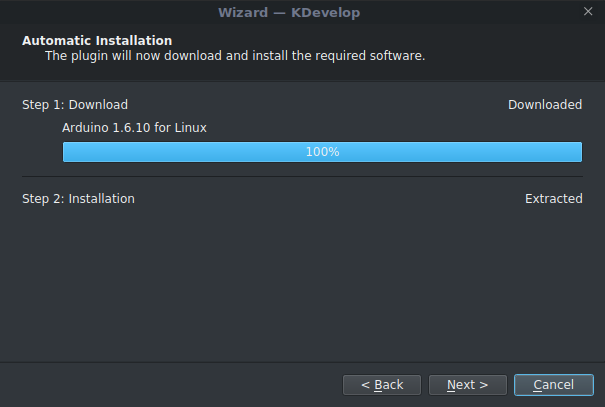
\includegraphics[width=0.85\textwidth]{figuras/kdevelopInstaller22.png}
\end{figure}

\begin{figure}[!htb]
  \centering
  \caption[End Configuration]{End Configuration}
  \label{fig:kdevelopinstaller3}
  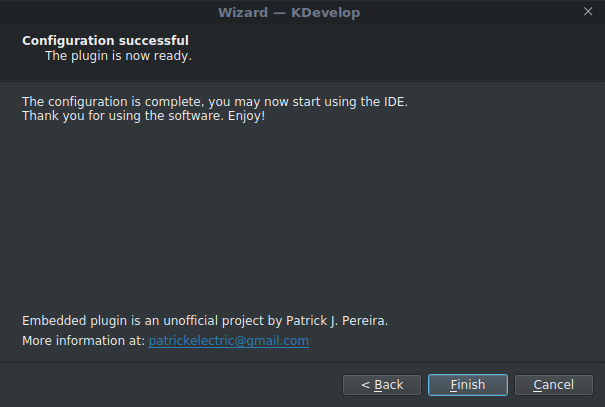
\includegraphics[width=0.85\textwidth]{figuras/kdevelopInstaller3.png}
\end{figure}

\subsection{Board Settings}

Interface para realizar o envio do binário para o sistema embarcado, permitindo o usuário interagir com o sistema, escolhendo a placa e algumas opções simples como processador, frequência, interface de comunicação, tipo de log de dados da saída do \textit{bootloader}. Além de permitir visualizar e mostrar quais opções foram selecionadas (\figref{fig:boardsettings}).

\begin{figure}[!htb]
  \centering
  \caption[Board Settings com configuração inicial]{\textbf{Board Settings} sem configuração prévia.}
  \label{fig:boardsettings}
  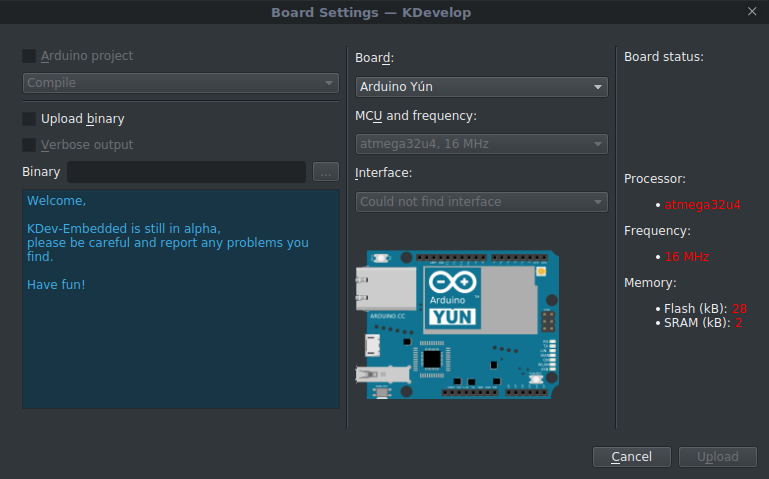
\includegraphics[width=0.85\textwidth]{figuras/boardsettings.png}
\end{figure}

Após ter o acesso a interface, o usuário pode escolher a opção de \textit{Upload Binary}, selecionando desta forma um arquivo contendo o código de maquina (\textit{Blink.hex}), após isso, pode-se escolher no menu \textit{Board} a placa para programar, permitindo ao plugin selecionar as opções para o hardware indicado, além disso, é necessário selecionar o tipo de processador e clock, como consta no menu \textit{MCU and frequency}, tendo isto selecionado, a ultima configuração necessária para realizar o envio do código é a porta que consta no menu \textit{interface}. Essas configurações podem ser visualizadas na \figref{fig:boardsettingsserial}, onde foi escolhido um Arduino Nano contendo um processador atmega328p com um clock de $16MHz$ utilizando uma interface de programação \textit{FT232 USB UART}.

\begin{figure}[!htb]
  \centering
  \caption[Board Settings após configuração para envio]{\textbf{Board Settings} após configuração do usuário.}
  \label{fig:boardsettingsserial}
  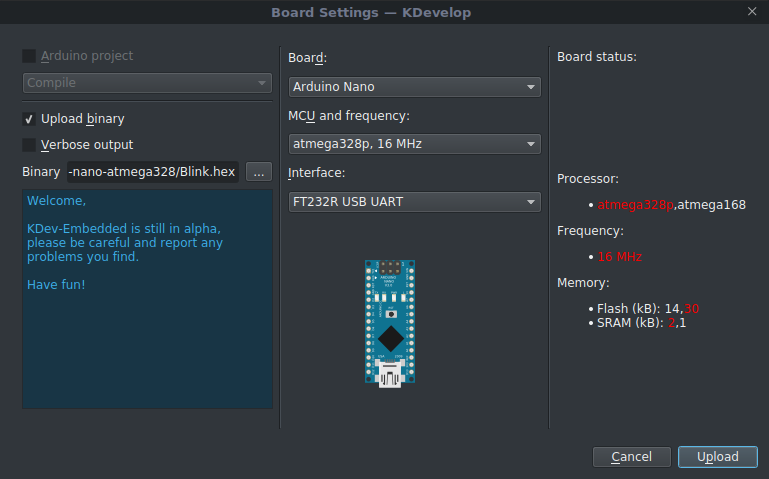
\includegraphics[width=0.85\textwidth]{figuras/boardsettingsSerial.png}
\end{figure}

Depois de tudo configurado, é possível clicar no botão \textit{upload} e realizar o envio do binário selecionado para placa. Podendo acarretar no sucesso da operação (\figref{fig:boardsettingsdone}) ou na sua falha (\figref{fig:boardsettingsndone}).

\begin{figure}[!htb]
  \centering
  \caption[Board Settings com sucesso no envio]{\textbf{Board Settings} após o envio do código para o sistema embarcado.}
  \label{fig:boardsettingsdone}
  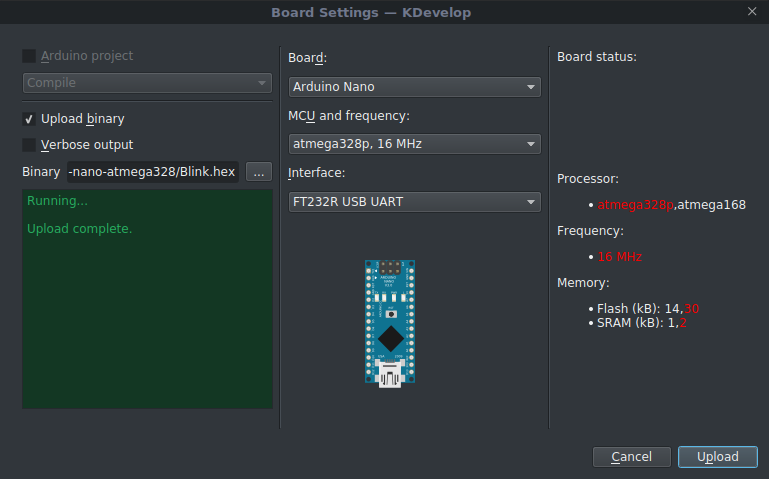
\includegraphics[width=0.85\textwidth]{figuras/boardsettingsdone.png}
\end{figure}

\begin{figure}[!htb]
  \centering
  \caption[Board Settings com falha no envio]{Imagem do \textbf{Board Settings} após falha no envio do código para o sistema embarcado.}
  \label{fig:boardsettingsndone}
  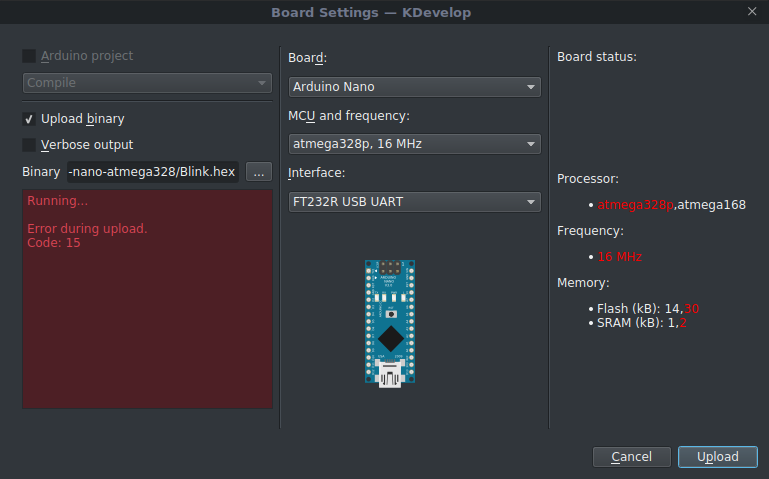
\includegraphics[width=0.85\textwidth]{figuras/boardsettingsndone.png}
\end{figure}

\section{Integração com fluxo de trabalho}
Além do desenvolvimento do software, permitindo seu uso como projetado inicialmente, foi necessário reservar uma parte do período do projeto para modificações de interface gráfica e de organização de layout, permitindo um uso simplificando para usuários não tão avançados, e ao mesmo tempo uma flexibilidade aos usuários com conhecimento profundo do funcionamento do sistema, modificando e personalizando as opções fornecidas pelo ambiente gráfico, sem restringir o alto nível de abstração que essas ferramentas já permitem.

\subsection{Integração e compilação do projeto}

Para realizar o usuário realizar compilação, é necessário importar um projeto: Project $\rightarrow$ Open / Import Project... e importe um projeto com um sistema de compilação suportado pelo KDevelop, seguindo o fluxo de trabalho do KDevelop (\figref{fig:importproject}).

\begin{figure}[!htb]
  \centering
  \caption[Import Project]{Import Project.}
  \label{fig:importproject}
  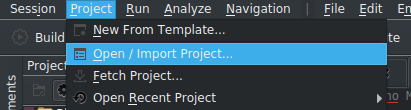
\includegraphics[width=1\textwidth]{figuras/importproject.png}
\end{figure}

Após o projeto ser importado com sucesso, será possível visualizar o mesmo no menu de projeto (\figref{fig:projects}).

\begin{figure}[!htb]
  \begin{minipage}[t]{0.5\textwidth}
  \caption[Projects antes da compilação]{Dock Projects antes\\ da compilação do projeto.}
  \label{fig:projects}
  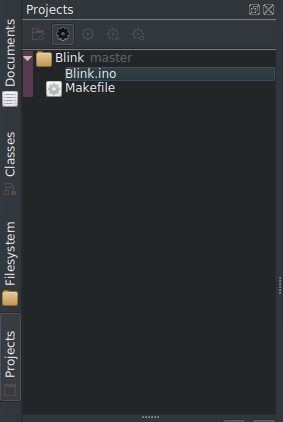
\includegraphics[width=0.7\textwidth]{figuras/projects.png}
  \end{minipage}%
  \begin{minipage}[t]{0.5\textwidth}
%  \raggedleft
  \caption[Projects depois da compilação]{Dock Projects depois\\ da compilação do projeto.}
  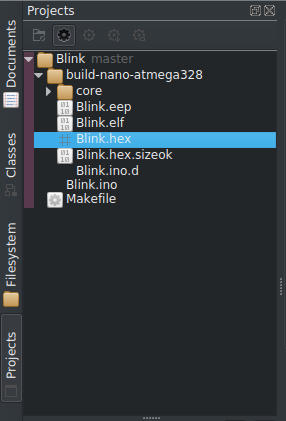
\includegraphics[width=0.713\linewidth]{figuras/projects2.png}
  \label{fig:projects2}
  \end{minipage}
\end{figure}

Depois de ter realizado a importação com sucesso, é necessário realizar a compilação para gerar o binário que será enviado pro processador, realizando o processo de compilação, basta clicar no botão \textit{Build} da interface do KDevelop, após isso, o menu de projeto se atualizado, podendo ser possível visualizar o arquivo com o código de maquina (\figref{fig:projects2}).

\subsection{Lançamento}

Seguindo o fluxo de trabalho do KDevelop, é necessário configurar o projeto para ser realizado o lançamento de uma forma correta. Para tal, basta executar Run $\rightarrow$ Configure Launchs (\figref{fig:run}).

\begin{figure}[!htb]
  \centering
  \caption[Configure Launchs]{Configure Launchs.}
  \label{fig:run}
  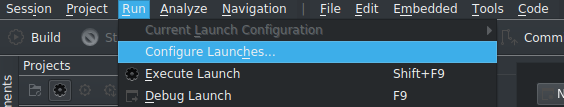
\includegraphics[width=1\textwidth]{figuras/run.png}
\end{figure}

Após isso, uma tela de configuração será aberta, podendo ser configurado da seguinte forma para um sistema embarcado, Add New... $\rightarrow$ Embedded e modificando o sistema de acordo com o alvo que será programado, \figref{fig:run2}. Nesta, foi utilizado um \textit{Arduino Nano} para realizar o teste de envio de código, também é possível selecionar a opção de \textit{OpenOCD} desenvolvido (\figref{fig:openocd}).

\begin{figure}[!htb]
  \centering
  \caption[\textit{Configure Launchs} para \textit{avrdude}]{Configure Launchs para \textit{avrdude}.}
  \label{fig:run2}
  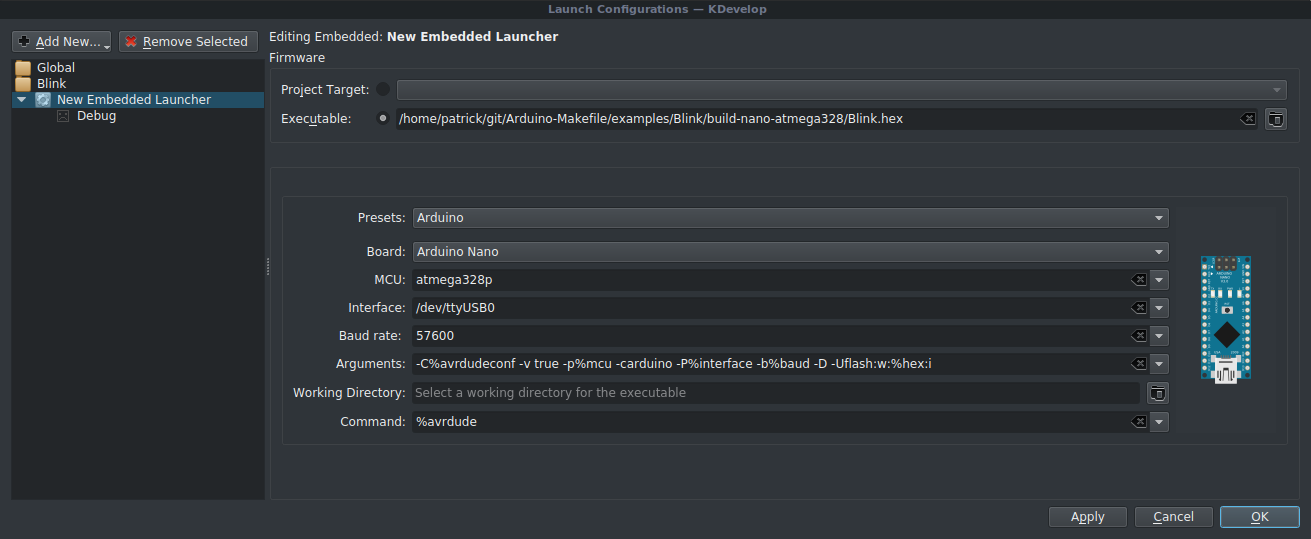
\includegraphics[width=1\textwidth]{figuras/run2.png}
\end{figure}

\begin{figure}[!htb]
  \centering
  \caption[\textit{Configure Launchs} para \textit{OpenOCD}]{Configure Launchs para \textit{OpenOCD}.}
  \label{fig:openocd}
  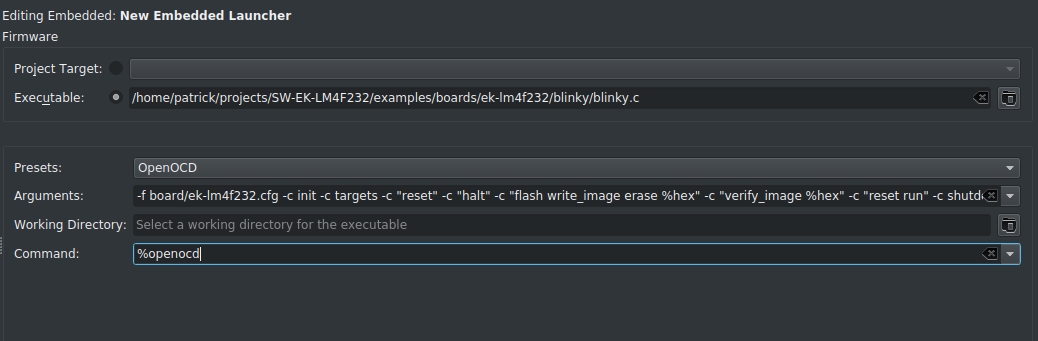
\includegraphics[width=1\textwidth]{figuras/openocd.png}
\end{figure}

Após realizar as configurações, basta aplica-las e em seguida executar o lançamento com o botão Execute. Tendo isso realizado, será aberto um console onde todos os dados de gravação serão mostrados (\figref{fig:runavrdude} e \figref{fig:runopenocd}).

Com as configurações salvas no lançador do código, as mesmas ficam reservadas num arquivo conhecido como *.kdev4, responsável por gerenciar os arquivos de configuração, permitindo que os próximos lançamento sempre utilizem as mesmas configurações, além de permitir outras configurações de lançamento em paralelo.

\begin{figure}[!htb]
  \centering
  \caption[\textit{Embedded Launcher} com \textit{avrdude}]{Embedded Launcher com saída do \textit{avrdude.}}
  \label{fig:runavrdude}
  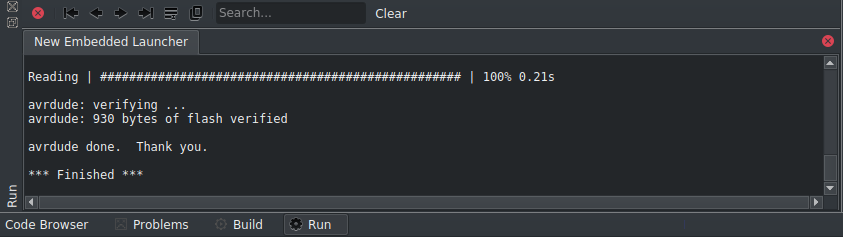
\includegraphics[width=1\textwidth]{figuras/runavrdude.png}
\end{figure}

\begin{figure}[!htb]
  \centering
  \caption[\textit{Embedded Launcher} com \textit{openocd}]{Embedded Launcher com saída do \textit{openocd.}}
  \label{fig:runopenocd}
  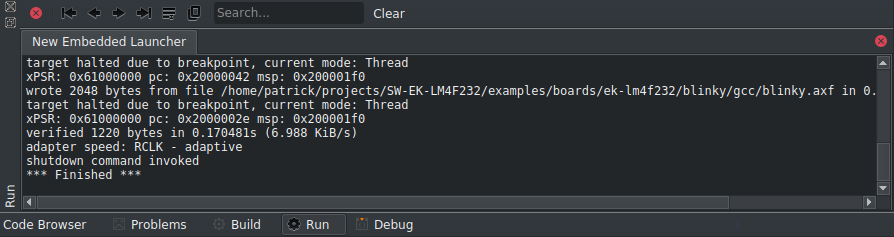
\includegraphics[width=1\textwidth]{figuras/runopenocd.png}
\end{figure}

\subsection{Depuração}

A depuração pode ser utilizada as próprias ferramentas do KDevelop, permitindo uma conexão com o servidor do GDB pela porta padrão, tal configuração foi testada utilizando a implementação do \textit{OpenOCD} (\figref{fig:openocddebug}).

\begin{figure}[!htb]
  \centering
  \caption[\textit{Debug mode} com \textit{openocd} no KDevelop]{\textit{Debug mode} com \textit{openocd.} no KDevelop}
  \label{fig:openocddebug}
  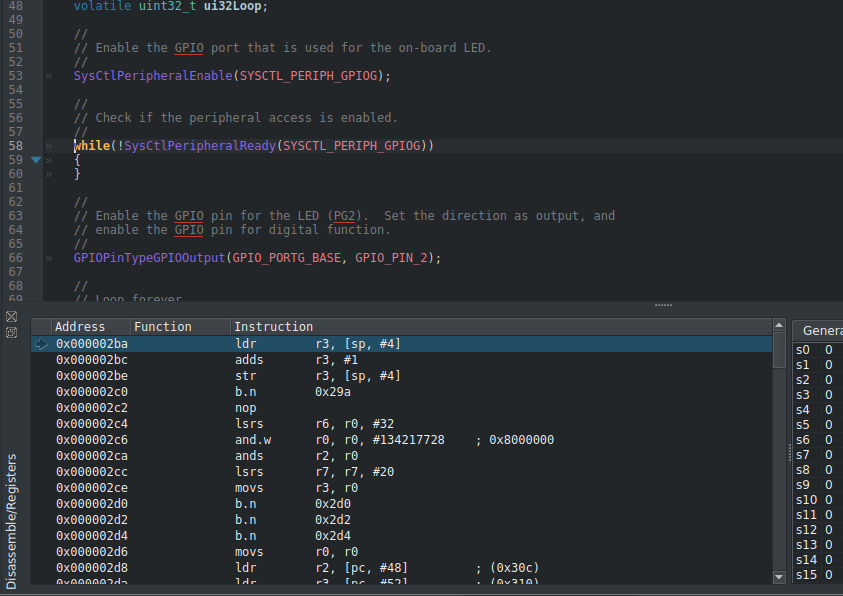
\includegraphics[width=0.85\textwidth]{figuras/DEBUG.png}
\end{figure}
